\subsubsection{Intel Xeon}
\par{ {\color{red}Intel Xeon E5-2660 v2 (Ivy Bridge): Vector Arithmetic Unit with 256-bit SIMD vectors.}}

\par{The kernel is dealing with calculations on single-precision floating-point. 
    Each floating point number is of size 32 bits (4 byte). Therefore there needs 
    to be at least 8 work items in dimension 0 for every work group. The hardware 
    requires this in order to fully utilize vectorization in the SIMD vector units. 
    Any lower than this results in under utilization of data parallelism, {\color{red}as can be seen 
    clearly from the graph trends of both capsid and nucleosome in figure \ref{nbody_xeon}.}}

\begin{figure}[!h]
    \centering
    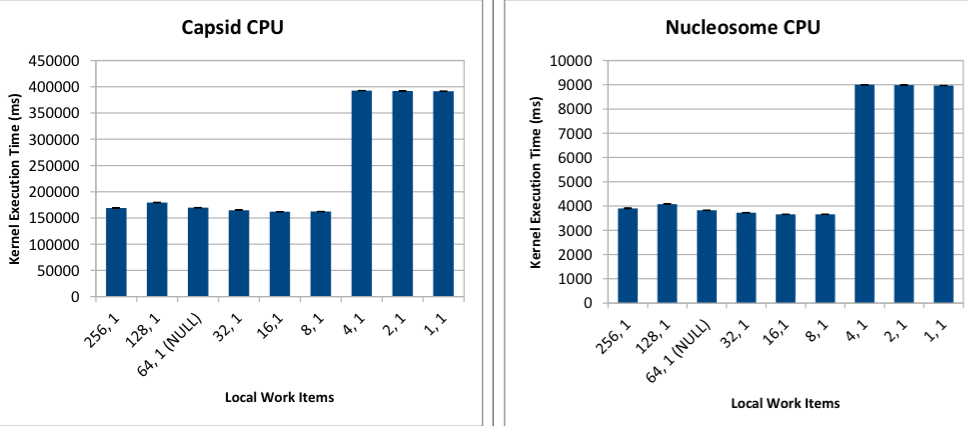
\includegraphics[width=0.8\textwidth]{figures/nbody_xeon.png}
    \caption{Graphical trends Nbody problem, Capsid and Nucleosome on Xeon.}
    \label{nbody_xeon}
\end{figure}

\par{From the profiler results in figure \ref{nbody_vtune}, 
    it is clear that this kernel is a good fit for parallel computing. 
    For the majority of the total run time, most of the 40 cores are being used in the CPU. 
    The small amount of time spent with only 1 core running is likely due to the host and other 
    code which are required for this calculation.}

\begin{figure}[!h]
    \centering
    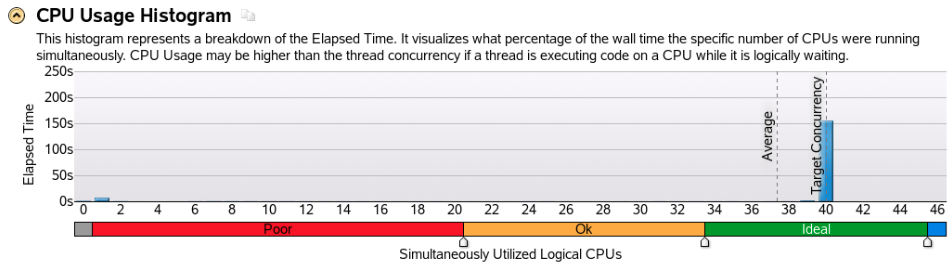
\includegraphics[width=0.8\textwidth]{figures/nbody_vtune.png}
    \caption{Vtune CPU usage histogram, nbody problem.}
    \label{nbody_vtune}
\end{figure}

\subsubsection{Intel Xeon Phi}
\par{{\color{red} Intel Xeon Phi 5110P: Vector Arithmetic Unit with 512-bit SIMD vectors.}}

\par{The same logic can be applied to the Xeon Phi. The only difference
    is that the Phi has larger vector units than the CPU. Hence, there needs 
    to be 16 work items in dimension 0 per work group. Graphs in figure \ref{nbody_phi} show this.}

\begin{figure}[!h]
    \centering
    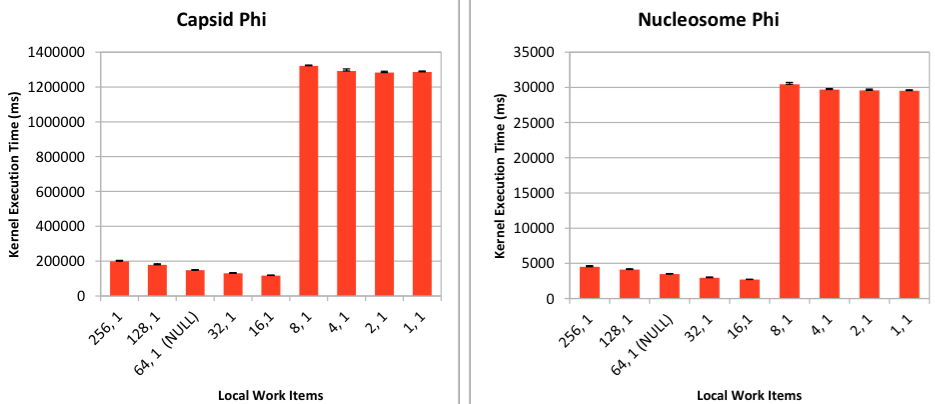
\includegraphics[width=0.8\textwidth]{figures/nbody_phi.png}
    \caption{Graphical trends Nbody problem, Capsid and Nucleosome on Xeon Phi.}
    \label{nbody_phi}
\end{figure}

\par{Figure \ref{nbody_phi_vec} clearly shows that the vector intensity with 16 work items is the greatest. 
    The same results must be occurring on the CPU as we see a very similar trend in the graphs. 
    The high vectorization values can be attributed to the regular access patterns of the kernel 
    and the OpenCL compiler.}

\begin{figure}[!h]
    \centering
    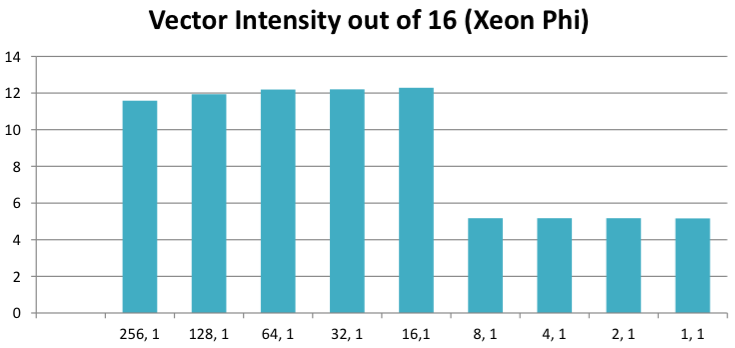
\includegraphics[width=0.8\textwidth]{figures/nbody_phi_vec.png}
    \caption{Vtune vector intensity Xeon Phi, Nbody.}
    \label{nbody_phi_vec}
\end{figure}

\par{Vtune results also showed that the values of 8 and 16 work items for the CPU and 
    Xeon Phi respectively had the lowest CPI rate. The CPI value of an application or 
    function is an indication of how much latency affected its execution. 
    Higher CPI values mean there was more latency in your system – on average, 
    it took more clockticks for an instruction to retire. 
    Latency in your system can be caused by cache misses, I/O, or other bottlenecks.}

\par{{\color{red}
    (https://software.intel.com/en-us/articles/intel-vtune-performance-analyzer-basics-what-is-cpi-and-how-do-i-use-it) 
    The higher L1 Hit Ratio can be seen in the Figure \_ later.}}

\subsubsection{GPU, Nvidia Tesla K20}
\par{{\color{red}Max. Compute Units: 13, Number of CUDA cores: 2,496, Therefore, each compute unit consists of 192 cores}}

\par{In Best case scenario, we have enough Work Groups to utilize all Streaming Multiprocessors(SM), 
    and also utilise all the cores within due to enough local work items.{\color{red}120 WG > 13 Compute Units,
    256 WI > 192 cores within each SM (compute unit)}}

\par{In the worst case scenario, we have enough Work Groups to utilise all the SM's 
    but the cores inside the SMs are empty due to little amount of local work items.{\color{red}
    The results on the GPU are shown in figure \ref{nbody_gpu}}}

\begin{figure}[!h]
    \centering
    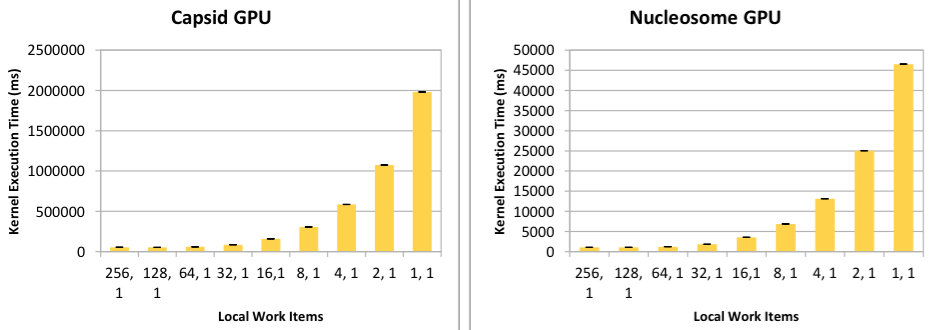
\includegraphics[width=0.8\textwidth]{figures/nbody_gpu.png}
    \caption{Graphical trends Nbody problem, Capsid and Nucleosome on GPU.}
    \label{nbody_gpu}
\end{figure}
        
\subsubsection{Comparision between all three hardwares}
\par{{\color{red}Figure \ref{nbody_comp} shows that} the GPU emerges as the hardware with the greatest performance. 
    This can be explained by the fact that the GPU has up to 64KB Configurable Shared Memory and L1 Cache.
    Since the memory access pattern of this kernel is coalesced (explained further on), having sufficient 
    first level cache is a key contributor to good performance. The Tesla K20 also has a peak theoretical 
    performance of 3.52 Teraflops, which is almost twice the rate for the Xeon Phi (~2 Tflops). 
    Also, due to the inherent level of parallelism in the kernel, the GPU is a great fit with 
    its greater length SIMD processors and native support for parallelism with a large number of threads.}

\par{As with the CPU and Xeon Phi, it is immediately apparent that the Xeon Phi 
    has a much greater degree of response to the under utilisation of vector units. 
    This is because the CPU is a smarter hardware which has better support for 
    serialized code in terms of branch prediction and a more sophisticated 
    memory management system.}

\begin{figure}[!h]
    \centering
    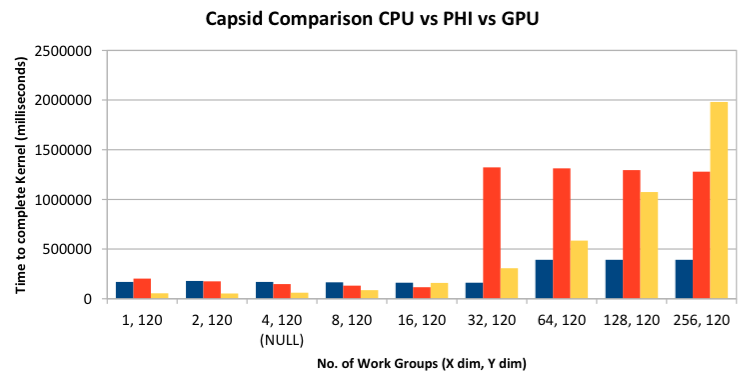
\includegraphics[width=0.8\textwidth]{figures/nbody_comp.png}
    \caption{Graphical trends Nbody problem, Capsid and Nucleosome comparison between architectures.}
    \label{nbody_comp}
\end{figure}

